\section{Conception}

Avant la conception du projet il est nécessaire la prise en main du logiciel VLAB et l'utilisation des toolbox disponibles comme le toolbox CAN, Ethernet, LIN et aurix. J'ai d'abord installé l'environnement du travail avec les identifiants pour accéder à la réseaux interne de la société. Deuxièmement, j'ai téléchargé les dossiers du travail depuis les servers d'Australie. Apr\`es, j'ai compil\'e du logiciel simple pour tester le microcontr\^oleur (désormais appel\'e \textit{aurix}). Finalement, j'ai modélisé quelques composants génériques pour tester des autres fonctionnalités du VLAB comme les connections des bancs de test, l'envoie de données à travers des différents réseaux et la réception et utilisation de données. Le développement de ce projet a \'et\'e divis\'e en 3 parties en fonction de l'évolution du même. 

\begin{itemize} 

    \item - Premier démo technique qui sers a faire la prise en main d'AUTOSAR, VLAB et l'environnement en général. 

    \item - Développement de l'aurix \textit{TC37xEXT}\cite{aurix.tc37e}, pas support\'e jusqu'\`a moment du démarrage du stage. 

    \item - Virtualisation du Gateway 

\end{itemize} 

\subsection{Premier d\'emo technique}

Le premier exemple est fait pour tester le logiciel avec une configuration super simple. Il consiste a envoyer une trame CAN et le SWC la renvoie vers le CANID source. Pour cet exemple une ECU générique a \'et\'e modélisé pour recevoir des trames CAN et LIN. Sur la figure \ref{fig:first-demo-diagram} se montre un diagrame de block des communications. Le code de ces ECUs se trouve dans l'anexe \ref{anexe:first_demo:hybrid_node}. Le code pour démarrer la simulation se trouve dans l'anexe \ref{anexe:first_demo:run_file}. 


\begin{figure}[!htb] 
\centering 
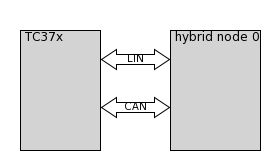
\includegraphics[]{img/first_demo_testbench.png} 
\caption{Premier démo. Codes dans l'annexe \ref{anexe:first_demo:testbench}.} 
\label{fig:first-demo-diagram} 
\end{figure} 

Le structure de communications d'AUTOSAR de la figure \ref{fig:autosar-com-stack} nous montre que le chemin parcouru par les données arrivant \'a l'aurix. Le chemin des données de cette première démo est le suivant \textit{Microcontroler}$ ->$ \textit{CAN\_Driver}\cite{can_drv_man} $->$ \textit{CAN\_IF}\footnote{IF dans la notation AUTOSAR veut dire Interface}\cite{can_if_man} $->$ \textit{PDU-R}\footnote{PDU est le nom des donn\'ees dans cette couche d'abstraction selon le modèle OSI\cite{osi-model}.}\footnote{PUD-R\cite{pdu_r_man} est le router des PDUs. C'est ce module qui prend le décision o\`u envoyer les données reçues}\cite{pdu_r_man}. C'est ici dans le PDU-R qu'on trouve un problème parce que la trame reçue n'est pas active au début du programme. 

Cette première démo a été conçue pour être teste avec le logiciel \textbf{CANoe}\cite{canoe} dont nous ne possédions pas la licence et le SWC n'a pas marché comme attendu. Les possibles explications sont les suivantes : 

\begin{itemize} 
    \item - Un protocole inconnu : Même si CANoe utilise le protocole CAN, il envoie peut-être d'autres trames d'identification avant le test. 
    \item - Un SWC peu test\'e : Selon la documentation de ce test, ce SWC n'a pas \'et\'e teste au fond parce que son utilisation ne sera jamais implémentée, c'est juste un test des logiciels. 

\end{itemize} 

\begin{figure}[!htb] 
\centering 
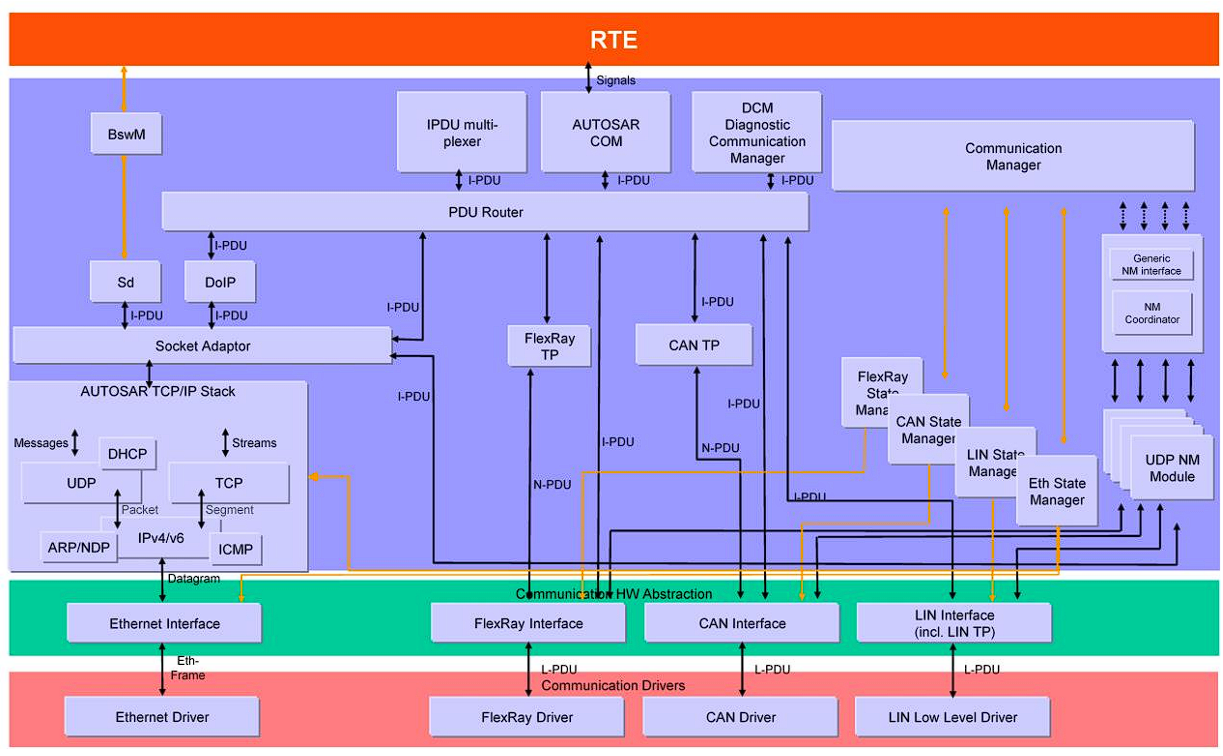
\includegraphics[width=\textwidth]{img/autosar_com_stack.png} 
\caption{Autosar Communication Stack\cite{sock_adp_man}} 
\label{fig:autosar-com-stack} 
\end{figure} 

Quand même, avec ce test j'ai acquis une connaissance basique du fonctionnement des logiciels AUTOSAR ce qui a rendu mon travaille future plus rapide et efficace. Une autre connaissance acquise dans cette partie c'était la partie de modélisation et le modèle de ECU déjà développe sera utilisé plus tard. 

\subsection{TC37xEXT} 

  

Cette version de l'aurix ajoutait quelques modules de plus, les plus concernant pour ce projet c'étaient une interface CAN (MCMCAN\footnote{C'est le nom de l'interface CAN dans la famille de microcontrôleurs \textit{aurix}}) et Gigabit Ethernet (GETH) de plus. Les autres différences seront trouvées dans la table \ref{tab:tc37x_delta}. Le modèle du \textit{TC37x}\cite{aurix.tc37x} a été pris comme la base et les interfaces et modules ont été ajout\'es selon les adresses de base sur les buses correspondantes. 


% Table generated by Excel2LaTeX from sheet 'Sheet1'
\begin{table}[htbp]
  \centering
    \begin{tabular}{|r||l|l|}
	\hline
	\multirow{2}{*}{Module} & \multicolumn{2}{c|}{Aurix}\\
	\cline{2-3}
	& TC37x & TC37xEXT \\
	\hline \hline
	    RAM & TRAM (cached, non-cached) & EMEM (cached, non-cached) \\
	    \hline
	    CAN interfaces & 2 & 3 \\
	    \hline
	    Camera Interface & not present & CIF \\
	    \hline
	    Gigabit Ethernet Interface & 1 & 2 \\
	    \hline
	    SD interface & not present & present \\
	    \hline
	    eMMC interface & not present & present \\
	    \hline
	\hline
    \end{tabular}
  \caption{TC37x Vs TC37xEXT}
  \label{tab:tc37x_delta}
\end{table}
 

Pour ce type de modélisation les informations sont fournies dans un fichier python qui fait l'assemblage de toutes les modèles de chaque module ou interface. Toutes les codes de cet assemblage dans l'annexe \ref{anexe:tc37ex:assembly}. Pour finaliser, il faut compiler et faire le test de chaque module ajout\'e. La compilation se fait avec la librairie \textit{Scons}\cite{scons} du python. Plus d'information à propos de ces codes dans l'annexe \ref{anexe:tc37ex:compilation}. 

Les tests doivent se faire en logiciel, il faut compiler un fichier \textit{.elf} et le monter sur la plateforme virtuelle créée et lancer un script de test qui vérifie si tout se passe bien. Dans le cas précis du \textit{TC37xEXT}, nous avons test\'e l'accès aux registres de mémoire ajout\'e et des interfaces MCMCAN et GETH. Les tests se trouvent dans l'annexe \ref{anexe:tc37ex:tests}. 

\subsection{Gateway Demo} 

  

Grace a tout le développement déjà fait démarrer cette simulation a été plus rapide. Les connections internes du Gateway sont montres dans la figure \ref{fig:devices-diagram}. A partir de cette configuration le testbench assemble se montre dans la figure \ref{fig:connections-diagram}.  

  

\begin{figure}[!htb] 

    \centering 

        \subfigure[Gateway Démo Devices \cite{gateway-pb}]{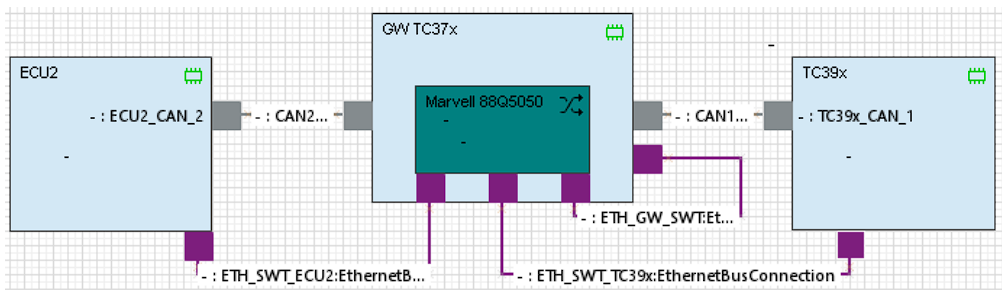
\includegraphics [width=5in]{img/GWDemoConnections.PNG}} 

        \subfigure[Details des connections Ethernet du Gateway]{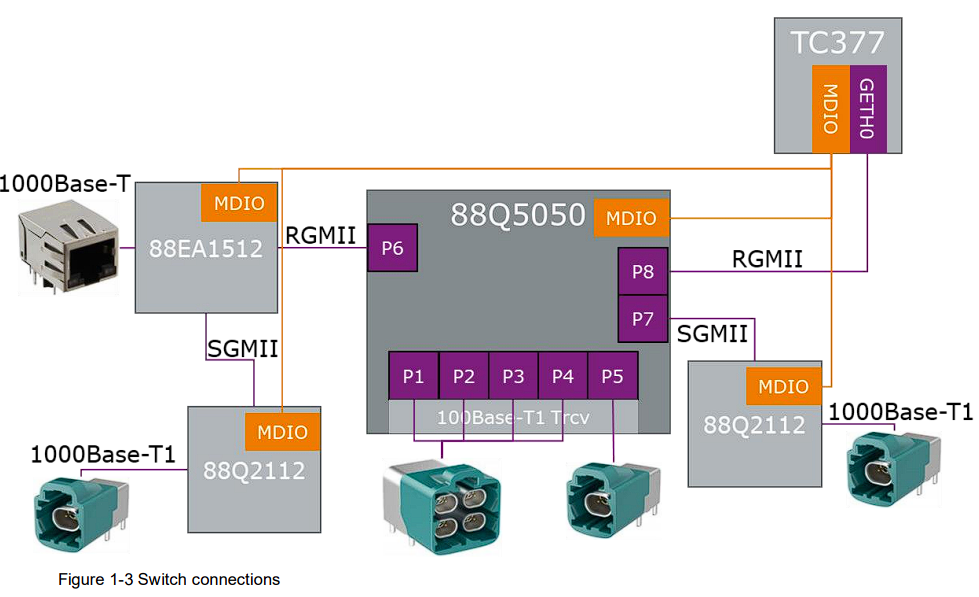
\includegraphics [width=5in]{img/eth_connections.png}} 

    \caption{Appareils de la démo technique} 

    \label{fig:devices-diagram} 

\end{figure} 

  

  

\begin{figure}[!htb] 

\centering 

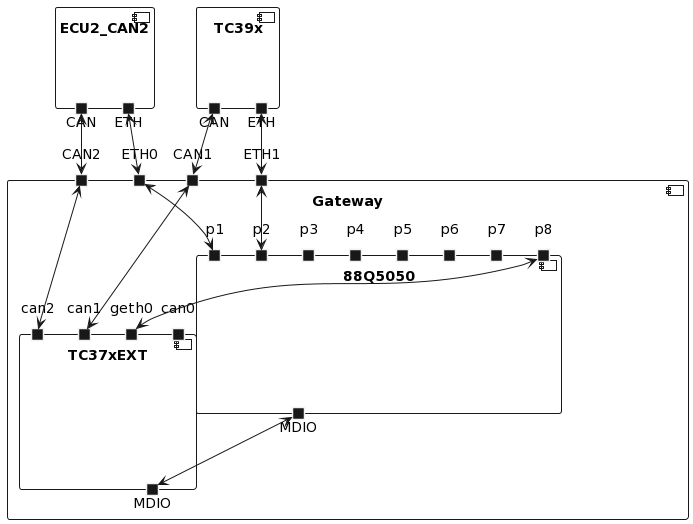
\includegraphics[width=\textwidth]{img/GWConnectionsDiagram.png} 

\caption{Gateway Connections Diagram, assemble avec le testbench de l'annexe \ref{anexe:gw_demo:testbench}} 

\label{fig:connections-diagram} 

\end{figure} 

  

\begin{figure}[!htb] 

\centering 

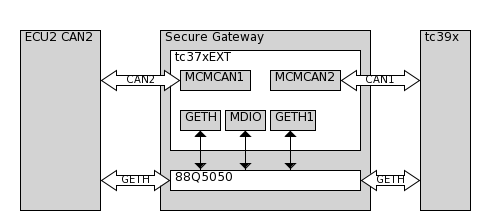
\includegraphics[width=\textwidth]{img/gateway_block_diagram.png} 

\caption{Gateway Block diagram} 

\label{fig:block diagram} 

\end{figure} 

  

\subsubsection{Switch Marvell 88Q5050} 

  

Avant de démarrer les SWC le logiciel de la Gateway vérifie si toutes les composants et buses de données sont présents. Un des composants présents dans la carte est le Switch Ethernet Marvell 88Q5050\cite{sw88Q5050}. C'est un switch sécurise optimise pour être utilise dans l'industrie automobile. Il est connecté aux ECUs externes via ports Ethernet et avec l'aurix a travers d'un port Ethernet et un bus MDIO\cite{mdio-background}. Ce bus MDIO est utilisé pour accéder aux registres du switch à travers de l'aurix. De cette façon nous pouvons gérer le fonctionnement interne du switch avec l'aurix. Comme ce n'est pas une méthode de communication habituelle j'ai dû développer un modèle de bus pour l'envoie de données a travers de ce bus en C++ avec systemC. L'implémentation se trouve dans l'annexe \ref{anexe:gw_demo:mdio_bus}. 

  

Le modèle du switch Ethernet a été développé en systemC aussi à l'aide de la datasheet du fournisseur. Pour ce modèle j'ai suivi la procédure interne de modélisation des composants en ajoutant la quantité de buses, registres, ports et fonctionnalités de chaque élément. Ce développement a des informations confidentielles donc il ne sera pas montre dans ce rapport. 

  

\subsubsection{Transceivers Marvell} 

  

Ces transceivers montr\'es dans la figure \ref{fig:devices-diagram}\cite{88Q2112}\cite{88Q1010} connectent la couche PHY avec le switch. Avant le démarrage du logiciel le système d'exploitation vérifie son statut pour initialiser les ports. 

  

Au moment de la rédaction de ce rapport, nous ne possédions pas les datasheets de ces transceivers. Dans le modèle du switch 88Q5050 est intégré les commandes nécessaires pour "initialiser les transceivers". 

  

La simulation est exécutée dans le fichier de l'annexe \ref{anexe:gw_demo:run_file}. 